%%%%%%%%%%%%%%%%%%%%%%%%%%%%%%%%%%%%%%%%%
% Beamer Presentation
% LaTeX Template
% Version 1.0 (10/11/12)
%
% This template has been downloaded from:
% http://www.LaTeXTemplates.com
%
% License:
% CC BY-NC-SA 3.0 (http://creativecommons.org/licenses/by-nc-sa/3.0/)
%
%%%%%%%%%%%%%%%%%%%%%%%%%%%%%%%%%%%%%%%%%

%----------------------------------------------------------------------------------------
%	PACKAGES AND THEMES
%----------------------------------------------------------------------------------------

\documentclass[xcolor=dvipsnames]{beamer}

\mode<presentation> {

% The Beamer class comes with a number of default slide themes
% which change the colors and layouts of slides. Below this is a list
% of all the themes, uncomment each in turn to see what they look like.

%\usetheme{default}
%\usetheme{AnnArbor}
%\usetheme{Antibes}
%\usetheme{Bergen}
%\usetheme{Berkeley}
%\usetheme{Berlin}
%\usetheme{Boadilla}
\usetheme{CambridgeUS}  
%\usetheme{Copenhagen}
%\usetheme{Darmstadt}
%\usetheme{Dresden}  
%\usetheme{Frankfurt}
%\usetheme{Goettingen}
%\usetheme{Hannover} 
%\usetheme{Ilmenau}
%\usetheme{JuanLesPins}
%\usetheme{Luebeck}
%\usetheme{Madrid}
%\usetheme{Malmoe}
%\usetheme{Marburg}
%\usetheme{Montpellier}
%\usetheme{PaloAlto}
%\usetheme{Pittsburgh}
%\usetheme{Rochester} 
%\usetheme{Singapore}
%\usetheme{Szeged}
%\usetheme{Warsaw}

% As well as themes, the Beamer class has a number of color themes
% for any slide theme. Uncomment each of these in turn to see how it
% changes the colors of your current slide theme.

%\usecolortheme{albatross}
%\usecolortheme{beaver}
%\usecolortheme{beetle}
%\usecolortheme{crane}
%\usecolortheme{dolphin}
%\usecolortheme{dove}
%\usecolortheme{fly}
%\usecolortheme{lily}
%\usecolortheme{orchid}
%\usecolortheme{rose}
%\usecolortheme{seagull}
%\usecolortheme{seahorse}
\usecolortheme{whale}
%\usecolortheme{wolverine}

%\setbeamertemplate{footline} % To remove the footer line in all slides uncomment this line
%\setbeamertemplate{footline}[page number] % To replace the footer line in all slides with a simple slide count uncomment this line

%\setbeamertemplate{navigation symbols}{} % To remove the navigation symbols from the bottom of all slides uncomment this line
}

\usepackage{graphicx} % Allows including images
\usepackage{booktabs}
\usepackage{amsmath}
\usepackage{amsfonts}
\usepackage{algorithm}
\usepackage{algorithmic}
\usepackage[utf8]{inputenc}
\usepackage{url}% for url's in bib
\usepackage{array}
\usepackage{epstopdf}
\usepackage{xcolor}
\usepackage[absolute,overlay]{textpos}
\usepackage{movie15}
\usepackage{media9}




%----------------------------------------------------------------------------------------
%	TITLE PAGE
%----------------------------------------------------------------------------------------

\title[Algorithms for controlling and tracking UAVs in indoor scenarios]{Algorithms for controlling and tracking UAVs in indoor scenarios} 

\author{Andrea Nisticò} % Your name
\institute[UNIGE] % Your institution as it will appear on the bottom of every slide, may be shorthand to save space
{
Supervised by: Marco Baglietto, Fulvio Mastrogiovanni \\
Co-supervised by: Tommaso Falchi Delitalia \\
\medskip
DIBRIS - Department of Informatics, Bioengineering, Robotics, and Systems Engineering \\
\smallskip
University of Genova
\medskip

Degree in \textit{Robotics Engineering} 
}
\date{September 18, 2015} % Date, can be changed to a custom date

% Restyling
\useinnertheme{rectangles}
\useoutertheme{infolines}
\setbeamertemplate{itemize items}[square]
\setbeamertemplate{enumerate items}[square]
\setbeamertemplate{title page}[default][rounded=false]
\setbeamertemplate{section in toc}[square]
\setbeamercolor{frametitle}{fg=Blue!80,bg=Gray!10}
\setbeamertemplate{blocks}[default]
\setbeamercolor{block title}{fg=Blue,bg=NavyBlue!20}
\setbeamercolor{block body}{fg=Black,bg=NavyBlue!5}
 \graphicspath{f/}

\begin{document}

\begin{frame}
\titlepage % Print the title page as the first slide
\end{frame}

\begin{frame}
\frametitle{Overview} 
\tableofcontents[sectionstyle=show,square]
\end{frame}

%----------------------------------------------------------------------------------------
%	PRESENTATION SLIDES
%----------------------------------------------------------------------------------------

%------------------------------------------------
\section{Introduction} 

\begin{frame}
\frametitle{The quadrotor}
The number of applications in which UAVs (Unmanned Aerial Vehicles) are involved is exponentially increasing, especially in indoor scenarios. \\~\\ 
The most popular architecture is the \textbf{quadrotor}: a helicopter
with four rotors. The main features are:\\ 

\begin{itemize}
\item Good stability
\item Omni-directional kinematics 
\item Hovering on a fixed point
\item Medium payload
\end{itemize}

\begin{textblock*}{5cm}(7cm,4.6cm) % {block width} (coords)
\includegraphics[width=0.8\textwidth]{f/quad.png}
\end{textblock*}

\vspace{2ex}
Due to its properties, the quadrotor is the main chosen architecture for indoor flight.
\end{frame}

%------------------------------------------------

\begin{frame}
\frametitle{Problem statement}
\begin{block}{Goal}
We want to design a set of algorithms and SW components enabling a quadrotor
to achieve stability, through position feedback given from a motion capture system,
and perform different tasks in an indoor scenario.
\end{block} 
The work of this thesis produced:
\begin{itemize}
\item A correct integration between the on board autopilot and the mocap system
\item A functioning experimental setup mounted in the new laboratory
\item A software architecture capable of letting the robot execute tasks sequentially from a list
\item A procedure for landing on a moving platform
\end{itemize}
\end{frame}

\begin{frame}
\frametitle{Work flow}

The total work is divided in main steps:
\begin{enumerate}

\item Analysis of state of the art approaches to UAV control and modeling

\item Technical analysis and documentation on the given tools (Autopilot, Motion Capture, Quadcopter)

\item Integration between mocap and the quadrotor
\begin{itemize}

\item Integration and testing between mocap and onboard estimation modules
\item Integration and testing of onboard controller through set point control

\end{itemize}
\item Relocation of the equipment in the new laboratory
\item Design of the high level software architecture 
\item Testing the software, coding and debugging different kind of tasks
\item Design and testing an algorithm for landing on a mobile platform

\end{enumerate}
\end{frame}

%------------------------------------------------

\section{System setup}
\begin{frame}
\tableofcontents[sectionstyle=show,square,currentsection]
\end{frame}


\begin{frame}
\frametitle{Setup}
We can identify five distinct parts:
\vspace{2em}
\begin{itemize}
\item  IRIS quadcopter from 3D robotics
\item  Motion Capture system from Optitrack
\item  Linux workstation
\item  Windows machine
\item  Flight arena
\end{itemize}
\end{frame}
%-------------------------------------------------
\begin{frame}
\frametitle{IRIS}
The IRIS quadcopter is flying robot manufactured by 3DRobotics and commercially available. \\~\\ 

	\begin{columns}[t]
		\column{.5\textwidth} 
		\textbf{Main features}
		\begin{itemize}
			\item Relatively cheap
			\item High quality and robust 
			\item Ready to fly
			\item Compatible with Android tablets
		\end{itemize}
		\column{.5\textwidth}
		\textbf{Main components}
		\begin{itemize}
			\item Four 850 KV motors ( PWM )
			\item One 11.1 V LiPo battery
			\item Control electronics
			\item Auto pilot software
		\end{itemize}
	\end{columns}
\end{frame}
%------------------------------------------------
\begin{frame}
\frametitle{IRIS}
\begin{figure}
\centering
\includegraphics[width = 0.5\textwidth]{f/iris.jpg}
\includegraphics[width = 0.5\textwidth]{f/iris_planner.jpg}

\end{figure}

\end{frame}
%----------------++--------------------------------
\begin{frame}
\frametitle{IRIS - PixHawk / PX4}
The brain of the robot is the \textbf{PixHawk} board. 
\begin{itemize}
\item Two embedded processors
\item IMU, barometer, magnetometer  and GPS receiver
\item ESCs (Electronic Speed Controllers) 
\item RC Radio interface
\item Telemetry module through MAVLink protocol
\end{itemize}
Featuring the \textbf{PX4} open source autopilot. \\~\\
PX4 runs on NuttX, an open source RTOS, and includes different modules executing in parallel. 
\\~\\
Modules implement: estimation and control, low level management, failsafe.
\end{frame}

%--------------------------------------------------
\begin{frame}
\frametitle{Motion Capture}
Responsible for the localization of the robot.\\~\\

It relies on eight OptiTrack cameras detecting IR beams reflected by passive markers. \\~\\

Provides 6D (translation and rotation) position of rigid bodies defined by at least three markers. Position is provided by a local frame predefined by the user. 
\begin{figure}
\centering
\includegraphics[width = 0.3\textwidth]{f/irismarker.jpg} \hspace{2em}
\includegraphics[width = 0.405\textwidth]{f/motiv_panorama.PNG}
\end{figure}
\end{frame}
%--------------------------------------------------
\begin{frame}[t]
\frametitle{Adapting reference frames}

\begin{columns}[t] % The "c" option specifies centered vertical alignment while the "t" option is used for top vertical alignment
\column{.45\textwidth} % Left column and width
\textbf{Mocap reference frame}
\begin{itemize}
\item X and Z axis on the horizontal plane
\item Y axis vertical pointing up

\end{itemize}
\column{.5\textwidth} % Right column and width
\textbf{Earth reference frame}
\begin{itemize}
\item X and Y axis on the horizontal plane
\item Z axis vertical pointing down
\item When mag is on, X is North, Y East and Z is down
\end{itemize}
\end{columns}

\begin{columns} % The "c" option specifies centered vertical alignment while the "t" option is used for top vertical alignment
\column{.5\textwidth} % Left column and width
\begin{equation*}
\begin{aligned}
P\textsuperscript{E}& = \begin{bmatrix}x&&z&&-y\end{bmatrix}^T
\\
Q\textsuperscript{E}& = \begin{bmatrix}
w&&x&&z&&-y
\end{bmatrix}^T\\
\end{aligned}
\end{equation*}

with $[x,y,z]$ and $[w,x,y,z]$ in mocap frame
\column{.5\textwidth}
\includegraphics[width = 1\textwidth]{f/frames.png}
\end{columns}
\end{frame}

\begin{frame}
\frametitle{Overall integration}
\begin{figure}
\centering
\includegraphics[width = 0.69\textwidth]{f/integration.png}
\end{figure}

\end{frame}

%--------------------------------------------------
\section{Modeling, estimation and control}

\begin{frame}
\tableofcontents[sectionstyle=show,square,currentsection]
\end{frame}

\begin{frame}[t]
\frametitle{Reference frames}
\begin{itemize}
\item $\Re^B$ body frame, attached to the robot center of mass
\item $\Re^E$ earth frame, placed on the floor at the center of the room
\end{itemize}
\begin{figure}
\centering
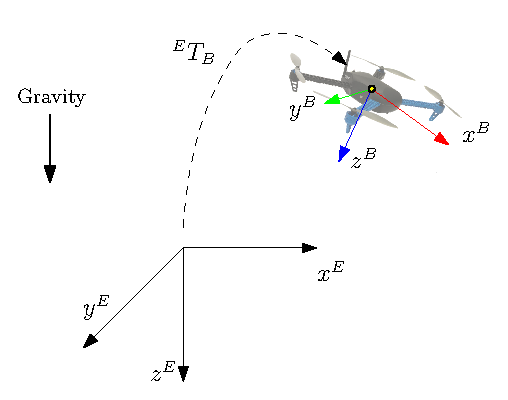
\includegraphics[width = 0.5\textwidth]{f/ref_frames.eps}
\end{figure}
${}^ET_B$ defines the transformation of $\Re^B$ respect to $\Re^E$ as base frame.
\end{frame}


\begin{frame}
\frametitle{Propulsion}
Each rotor generates:\begin{itemize}
\item A force $f_i = k \omega_i ^ 2$
\item A torque $\tau_i = k_d \omega_i ^ 2$
\end{itemize} 
Performing forces and torques balance:
\begin{equation*}
\begin{bmatrix}
T^B\\\tau_\phi\\\tau_\theta\\\tau_\psi
\end{bmatrix} = \begin{bmatrix}
k&&k&&k&&k\\
k d_i S(30)&&-k d_i S(30)k&& -d_i S(30)&&d_i S(30)\\
-k d_i C(30)&&-k d_i C(30)k&& d_i C(30)&&d_i C(30)\\
k_d&&-k_d&&-k_d&&k_d
\end{bmatrix} \begin{bmatrix}
\omega_1\\\omega_2\\\omega_3\\\omega_4
\end{bmatrix}^2
\end{equation*}
$T^B$: thrust along $z^B$ \\ $\tau$ : torques on the three axis
\end{frame}

\begin{frame}[t]
\frametitle{Rigid body equations}
The model is described by the well known rigid body equations of motion:
\begin{align*}
\boldsymbol{\dot{r}}& = \boldsymbol{v}\\ 
m\boldsymbol{\dot{v}}& = \boldsymbol{F}\\ 
\dot{R}& = R\Omega_\times\\ 
I\boldsymbol{\dot{\Omega}}& = -\boldsymbol{\Omega} \times I\boldsymbol{\Omega} + \boldsymbol{\tau}
\end{align*}
Define the input vector as : $\textbf{U} = \begin{bmatrix}
T^B&&\tau_\phi && \tau_\theta && \tau_\psi
\end{bmatrix}^T$
\vspace{2em}

then: $\boldsymbol{\dot{v}} = \frac{1}{m}\left(\begin{bmatrix}0\\0\\mg\end{bmatrix}^E + R\begin{bmatrix}0\\0\\U_1\end{bmatrix}^B\right)$  and $\boldsymbol{\dot{\Omega}} =I^{-1}\left(\begin{bmatrix}
U_2\\U_2\\U_4
\end{bmatrix} -\boldsymbol{\Omega} \times I\boldsymbol{\Omega}\right)$
\end{frame}

\begin{frame}[t]
\frametitle{State estimation}

\begin{columns}[t]
\column{.5\textwidth}
\textbf{Position estimator}:
Fixed gain observer
\begin{itemize}
\item Accelerometers (input)
\item GPS
\item Barometer
\item Mocap
\end{itemize}
\vspace{1em}
Position estimator model:
\begin{equation*}
\begin{aligned}
	\boldsymbol{x_k}(\boldsymbol{x_{k-1}}, dt , \boldsymbol{a})& = \boldsymbol{x_{k-1}} + \boldsymbol{v_k}dt + \frac{1}{2}\boldsymbol{a} dt^2 \\
	 \boldsymbol{v_k} ( \boldsymbol{v_{k-1}} ,\boldsymbol{a} , dt)& = \boldsymbol{v_{k-1}} + \boldsymbol{a}dt
	 \end{aligned}
\end{equation*}
\column{.45\textwidth}
\textbf{Attitude estimator}:
Extended Kalman Filter
\begin{itemize}
\item Accelerometer
\item Gyroscope
\item Magnetometer
\end{itemize}
\vspace{2em}
 The magnetometer gives the value of the magnetic field in robot frame along three axis. The yaw is normally calculated respect to the North-South line.
\end{columns}



\end{frame}

\begin{frame}[t]
\frametitle{Yaw correct estimation}

\begin{columns}[t]
\column{0.5\textwidth}
Measured mag. field in body frame:
\\
\vspace{1em}
$\boldsymbol{mag}^B = \begin{bmatrix}mag_x \\ mag_y \\ mag_z\end{bmatrix}$ 
\column{0.5\textwidth}
Fake mag. field in earth frame:
\\
\vspace{1em}
$\boldsymbol{mag^E}$ = $\begin{bmatrix}1\\ 0 \\ 0.4\end{bmatrix}^T$
\end{columns}
\vspace{1em}
Then we cut of the magnetometer sensor and replace $\boldsymbol{mag}^B$ with:
\begin{equation}
	 \boldsymbol{mag^B} = R^T \boldsymbol{mag^E}
\end{equation}
\vspace{1ex}

\textit{Roll} and \textit{Pitch} angles are estimated by the EKF. By passing the value of the \textit{Yaw} calculated by the mocap we are able to construct the $R$ matrix and inject the value of $\boldsymbol{mag^B}$ inside the estimator.
\end{frame}


\begin{frame}
\frametitle{Controller structure}
Two modules implement a cascade of P / PID controllers: \textbf{position control} module and \textbf{attitude control} module.
\begin{figure}
\centering
\includegraphics[width = 1\textwidth]{f/control_arch.png}
\end{figure}
\end{frame}

\begin{frame}
\frametitle{Results}
\begin{textblock*}{1\textwidth}(0.4cm,1cm)
	\begin{figure}
	\vspace{1em}
	\includegraphics[width = 0.5\textwidth]{f/x_conv.png}
	\includegraphics[width = 0.5\textwidth]{f/y_conv.png} \\
	\vspace{1ex}
	\includegraphics[width = 0.5\textwidth]{f/z_conv.png}
	\includegraphics[width = 0.5\textwidth]{f/yaw_conv.png}
	\end{figure}
\end{textblock*}
\end{frame}


%------------------------------------------------
\section{Software architecture}

\begin{frame}
\tableofcontents[sectionstyle=show,square,currentsection]
\end{frame}

\begin{frame}[t]
\frametitle{Definition}
\begin{block}{Definition}
A software architecture is an abstract view of a software system distinct from the details of implementation, algorithms, and data representation.
\end{block}

It is represented by a block diagram. Each block is independent with known in/out relation.
\vspace{1ex}

A well written software architecture should:
 \begin{itemize}
 \item Provide flexibility and adaptability
 \item Allow for interoperability 
 \item Provide control on the system
 \item Reduce maintenance time and cost
 \item Help developers improving the software
 \end{itemize}

\end{frame}

\begin{frame}
\frametitle{Goal}
The SW must:\begin{itemize}
\item Be expandable
\item Be flexible
\item Be able to control the robot by sending position feedback and set point
\item Execute sequentially a list of tasks predefined by the user
\end{itemize}

\vspace{2em}
\textbf{Note: }Position feedback and set point are vectors $P = \begin{bmatrix}
x\\y\\z\\yaw
\end{bmatrix}$
\end{frame}

\begin{frame}
\frametitle{Scheme}
\begin{figure}
\centering
\includegraphics[width = 0.9\textwidth]{f/nested_arch.png}
\end{figure}
\end{frame}

\begin{frame}[t]
\frametitle{Design Patterns}
How do we design the core modules?
\vspace{3em}
\begin{block}{Design Pattern}
The pattern is a description or template for how to solve a problem that can be used in many different situations.
\end{block}
The Pattern is the architectural style chosen among the available ones depending on the problem. 

\vspace{2em}
A \textbf{Behavioral design} is used for organizing each SW component.

\end{frame}

\begin{frame}[t]
\frametitle{Behavioral design in nature}
Inspired from animals

\begin{figure}
\centering
\includegraphics[width =0.4 \textwidth]{f/frog.jpg}
\includegraphics[width =0.4 \textwidth]{f/pigeot.jpg}
\end{figure}
\begin{columns}

\end{columns}

\end{frame}



\begin{frame}
\frametitle{Demo}
\begin{figure}
\includegraphics[width = 0.5\textwidth]{f/circle.png}
%\includemovie[poster]{0.5cm}{0.5cm}{v/circle_final.MP4} \\
\includegraphics[width = 0.5\textwidth]{f/multiland.png}
%\includemovie[poster]{0.5cm}{0.5cm}{v/multiland.MP4}

\end{figure}

%\includemedia[
% width=0.5\textwidth
%]{	\includegraphics[width = 0.5\textwidth]{f/z_conv.png}}{v/circle_final.MP4}

\end{frame}

%------------------------------------------------

\begin{frame}[fragile] % Need to use the fragile option when verbatim is used in the slide
\frametitle{Verbatim}
\begin{example}[Theorem Slide Code]
\begin{verbatim}
\begin{frame}
\frametitle{Theorem}
\begin{theorem}[Mass--energy equivalence]
$E = mc^2$
\end{theorem}
\end{frame}\end{verbatim}
\end{example}
\end{frame}


%------------------------------------------------
\section{Landing on a mobile platform}

\begin{frame}
\tableofcontents[sectionstyle=show,square,currentsection]
\end{frame}

%------------------------------------------------

\section{Conclusions}

\begin{frame}
\tableofcontents[sectionstyle=show,square,currentsection]
\end{frame}

\begin{frame}
\Huge{\centerline{Thank you}}
\end{frame}

%----------------------------------------------------------------------------------------

\end{document} 